% Chapter 2

\chapter{Method} % Write in your own chapter title
\label{Chapter:Method}
\lhead{Chapter 2. \emph{\steel}} % Write in your own chapter title to set the page header

\section{Why do we need a new modeling technique in galactic astrophysics.}
%What is missing: Massive galaxies, checks 
In this thesis we propose a new modelling technique further diversifying the range of semi-empirical models already used in the field. With the breadth of simulations and techniques already used any additional models must justify their existence by showing they can succeed where others cannot. The primary and the arguably largest shortcoming of all the galaxy modeling techniques is the trade-off between volume and resolution. So far this limitation has severely limited the ability of models to constrain against the massive galaxy population. The reliance on discrete halos from merger trees or n-body simulations limits the number of massive galaxies simulated in more traditional models, limiting the ability of models to compare with observations of massive galaxies found in comprehensive surveys. 

%How can a new model succeed where others haven't
\steel has been designed as a complementary tool to the other galaxy models. In this chapter we describe the gaps in the current modelling space and the design choices in steel designed to address these gaps.

\section{Designing to specification.}
%General format: Science problem and design solution 
\subsection{Volume vs. Resolution}
%Volume/resolution - statistical
The trade-off between volume (or number of galaxies) and resolution stems directly from computational limitations. High resolution simulations resolve orders of magnitude more small haloes than large, below $10^13.5$ the halo number density increases by just below 1 magnitude for each drop of one magnitude in mass, left panel Figure \ref{fig:SubHaloes_byz}. Given a computer has a limited memory and processing power there is an upper limit to the total number of haloes/galaxies that can be simulated, either increasing the volume or lowering the resolution will increase the total number of galaxies simulated and therefore one must come at the expense of the other. In Figure \ref{fig:Vol_v_Res} this is visualised showing the Baryon Mass Resolution against the Number of Galaxies for many hydrodynamical simulations. The along the diagonals that are parallel to the line that connects top left to bottom right there are lines of constant particle number which when all other factors are constant will correspond to computational power. The two shaded boxes show the simulations that explore two modelling regimes:
\begin{itemize}
    \item The 'zoom in' where resolution is favoured allowing for the analysis of small galaxies/haloes and the structures of larger galaxies/haloes.
    \item The 'box' where a box of a given volume is simulated to try and understand what the structures look like on the scale of the box, this sacrifices the resolution of smaller galaxies and haloes.
\end{itemize}

\begin{figure}[h]
    \centering
    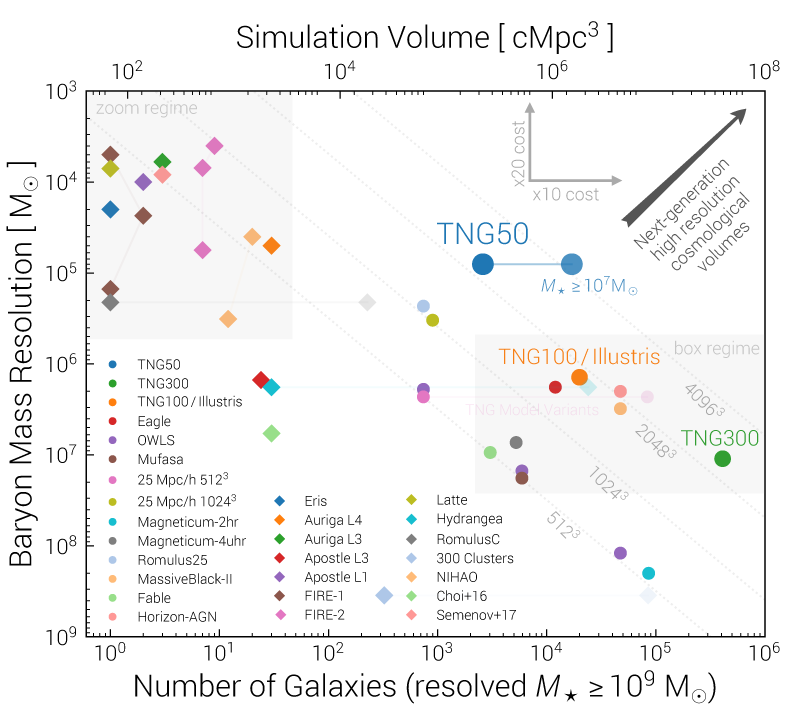
\includegraphics[width = \linewidth]{Figures/Chapter2/VolumeResolutionComparison.png}
    \caption{Image used with permission from: Illustris-TNG Project, \citet{Nelson2019FirstFeedback}}
    \label{fig:Vol_v_Res}
\end{figure}

In semi-analytic and semi-empirical models the analogous feature is found in the selection of merger trees fed to the models\footnote{For those semi-analytic/semi-empirical models that use n-body dark matter directly they follow the same pattern as the above but with dark matter particle resolution and number of haloes.} the number of haloes on a given merger tree is directly related to the lowest mass halo of interest. However, models using merger trees have one additional level of flexibility they can have a minimum subhalo mass and a minimum central halo mass. This provides flexibility in what can be simulated, for example:
\begin{itemize}
    \item High mass centrals, large box, high threshold for both central and subhalo mass. Suitable for exploring the evolution of massive galaxies.
    \item High mass centrals, medium/small box, low threshold for subhalo masses, moderate/high threshold for central masses. Suitable for exploring the environments around massive galaxies.
    \item Moderate/low mass centrals, medium/small box, low threshold for centrals and subhaloes. Suitable for exploring the evolution of large populations of smaller galaxies.
\end{itemize}


\steel has been specifically designed to not suffer from this trade-off by using a \textit{'Statistical Dark Matter Accretion history`} described in full in Section \ref{subsec:SDMAH}. In brief the statistical accretion histories follow the average growth of a given mass of halo backwards in time from $z = 0$. At each time-step the USHMF is assigned to the halo mass track by comparing the USHMF at t and t +$\Delta$t the subhalo accretion in $\Delta$t is calculated. The lifetime subhaloes is assigned using dynamical time arguments. This accretion history requires only the average halo mass tracks and the SHMF, each of which is a numerical quantity for each mass bin one mass track is calculated and scatter is implemented using the intrinsic statistical distributions of galaxies where appropriate. \steel therefore simulates massive haloes and small haloes equally and is able to produce massive rare galaxies in the same run as smaller galaxies whilst simulating neither with higher precedence.

%Flexibility - empirical
%Consistency - ensuring connections between high and low redshift
%Systematics - speed
\section{Modules and Methods}

\subsection{Statistical Dark matter accretion history}
\label{subsec:SDMAH}
%First we should explain merger trees and traditional simulation techniques.
\subsubsection{Traditional methods and merger trees}

%first n body
\begin{figure}[h]
    \centering
    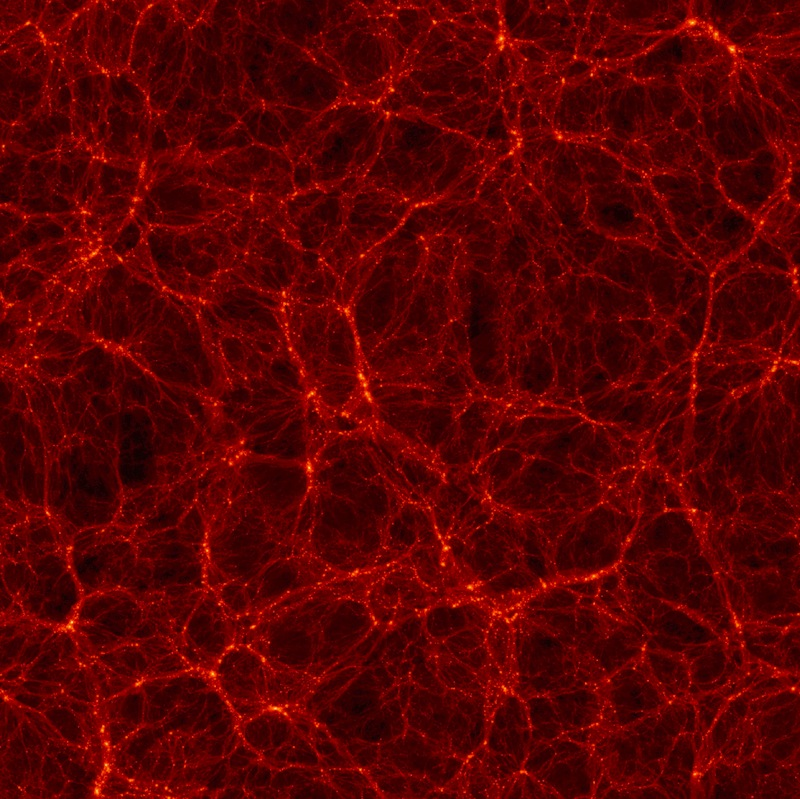
\includegraphics[width = \linewidth]{Figures/Chapter2/Bolshoi.jpg}
    \caption{Slice of the 250 Mpc$^3$ box of the Bolshoi Simulation. Brighter regions indicate a higher density of dark matter. Note the clustered bright points connected by large filaments. This structure is known as the cosmic web.
    Image credit: Bolshoi Simulation http://hipacc.ucsc.edu/Bolshoi/Images.html}
    \label{fig:Bolshoi}
\end{figure}

%then halofinders and trees (ROCKSTAR)

%then eps P08

%then hmf

%then shmf

\subsubsection{State of the art statistical method}
%then get onto what makes STEEL STEEL
\begin{figure}[h]
	\centering
	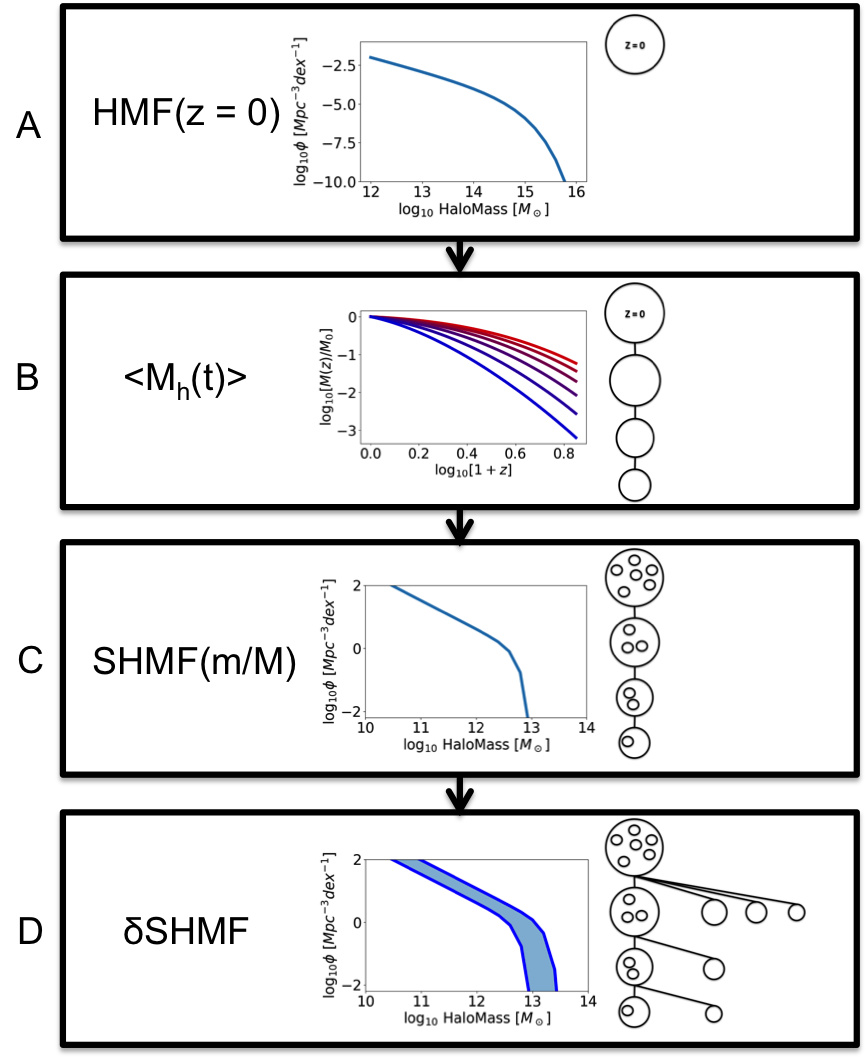
\includegraphics[width = \linewidth]{Figures/Chapter2/StatDM.png}
    \caption{I show the main steps in building the statistical dark matter accretion history for STEEL. Each panel shows a feature from a traditional merger tree and the statistical function used to replace it. A: The HMF is used to calculate the number densities of central haloes. B: Average mass growth histories are used to calculate the size of each mass bin at previous epochs. C: The (unevolved)SHMF is used to populate each central at each redshift with subhaloes. D: The average number densities of accreted subhaloes at each epoch, are calculated by taking the difference between each mass bin of the (unevolved)SHMF at consecutive redshift steps.}
	\label{fig:StatDM}
\end{figure}

\subsection{Abundance matching}
\label{C2:SubSec:AbnMtch}
\begin{figure}[h]
	\centering
	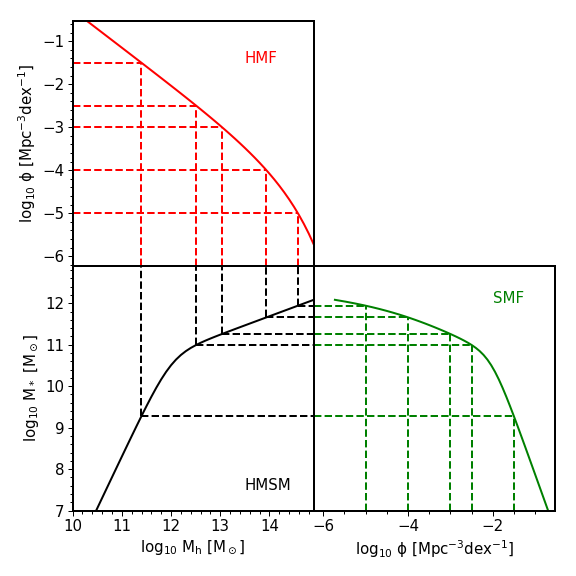
\includegraphics[width = \linewidth]{Figures/Chapter2/AbundaceMatching.png}
    \caption{A cartoon to show by matching the HMF (top left) and the SMF (bottom right) by abundance and the mapping between stellar and halo mass referred to as a SMHM relation (bottom left) is created.}
	\label{fig:Abn_Toon}
\end{figure}

\begin{figure}[h]
	\centering
	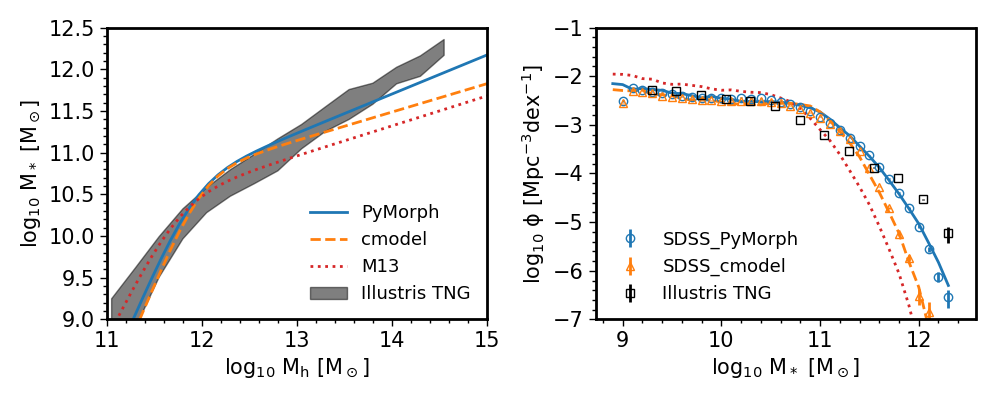
\includegraphics[width = \linewidth]{Figures/Chapter2/AbundaceMtch_Data.png}
    \caption{Left: The SMHM relation at redshift $z=0.1$. The PyMorph (blue solid line) and cmodel (orange dashed line) fits from this work are both for central haloes/galaxies, the fit from \citet{Moster2013} (M13, red dotted line) is for all haloes/galaxies. The grey band is the relation from Illustris TNG100. Right: Stellar mass functions created using the central halo mass function and the three SMHM relations compared to PyMorph (blue circles) and cmodel (orange triangles) central stellar mass functions. The black squares are the stellar mass function from Illustris TNG100.}
	\label{fig:Abn_Data}
\end{figure}

\subsection{Continuity star formation rate}
\begin{figure}[h]
	\centering
	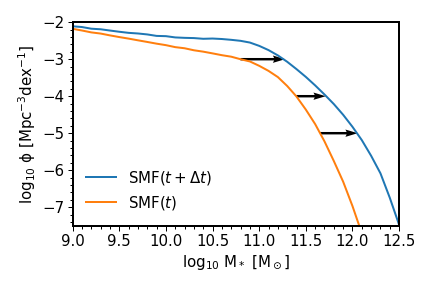
\includegraphics[width = \linewidth]{Figures/Chapter2/ContinuityEqn.png}
    \caption{The continuity approach connects at constant number density galaxy populations across cosmic time. Between two epochs `$t$' and `$t + \Delta t$' the SMF grows differently at different number density. The mass difference, $\Delta M$, indicated at three number densities by black arrows is the expected mass growth for each population.}
	\label{fig:Cont_Eqn}
\end{figure}

%Mass recycling

\begin{equation}
\label{eqn:f_ml}
f(\tau_{ml}) = 0.05 \ln \Big(\frac{\tau_{ml}}{1.4 Myr}+1\Big) ,
\end{equation}

\begin{equation}
\label{eqn:MLR}
MLR(t) = \frac{ \sum_{t' = t_{infall}}^{t} SFH(t')(f[t' - (t-\delta t)]-f[t' - t]) }{\delta t} .
\end{equation}

%Central Postprocessing 

%include a plot of using AM to convert HMGH to SMGH?
\begin{figure}[h]
	\centering
	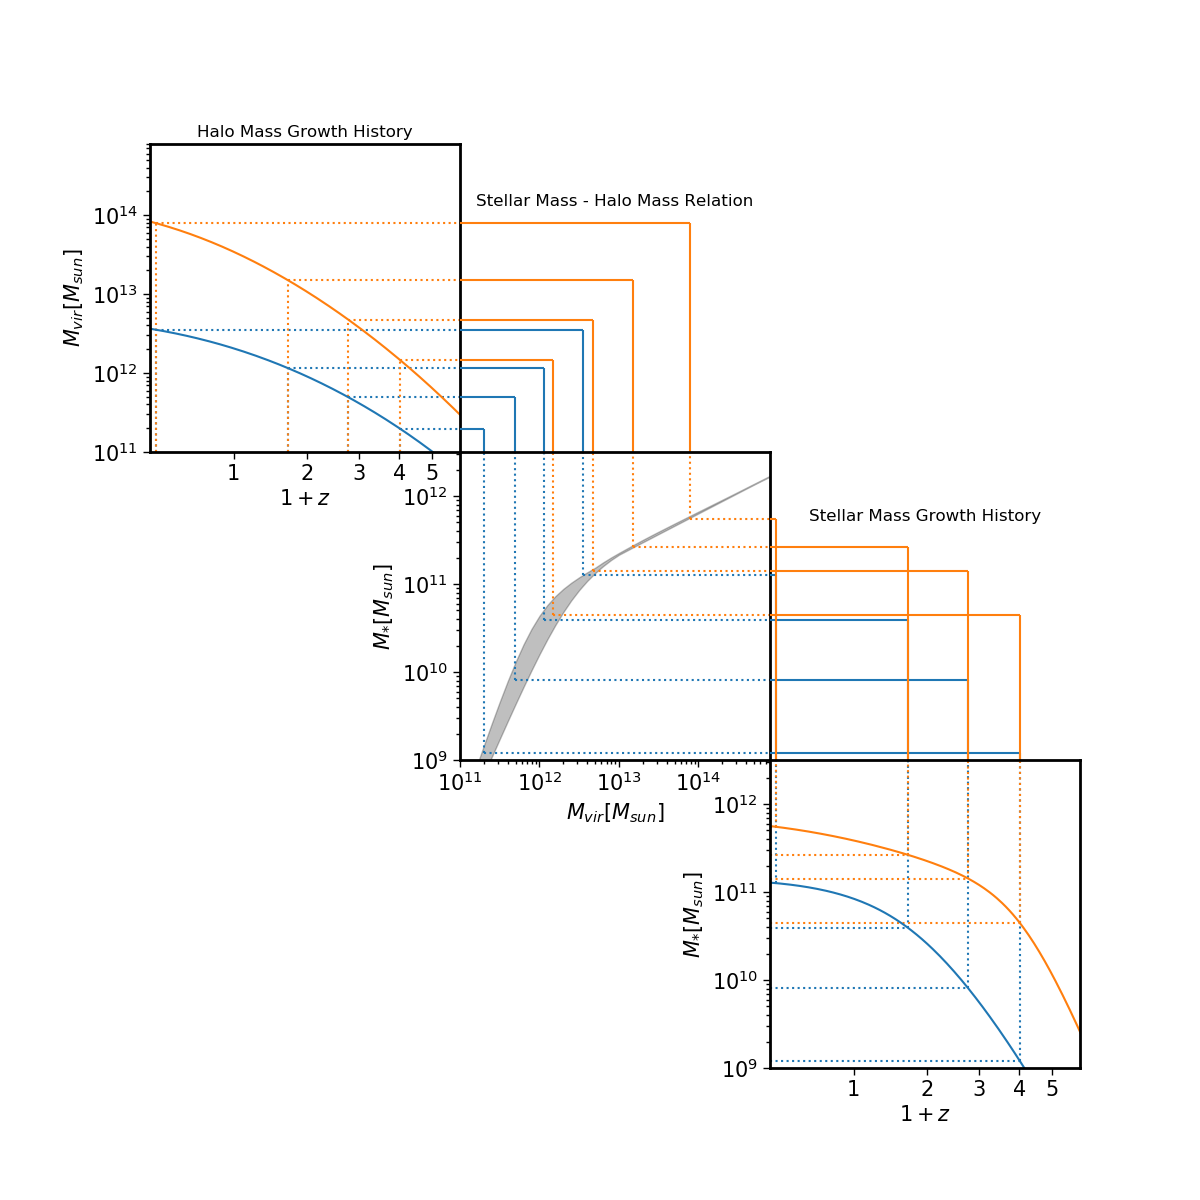
\includegraphics[width = \linewidth]{Figures/Chapter2/HMGH_to_SMGH.png}
    \caption{The Halo Mass Growth Histories (HMGH, top-left) are propagated though the redshift dependent stellar-mass-halo-mass relation (SMHM, middle) to produce corresponding Stellar Mass Growth Histories (SMGH, bottom-right). The lines illustrate matching points in redshift and the intersection with the SMHM relationship. The width of the SMHM relationship shows the extent of evolution with time, not as is common the scatter.}
	\label{fig:Cont_Eqn}
\end{figure}
